\documentclass[main.tex]{subfiles}

\begin{document}
\addtocontents{toc}{\let\protect\contentsline\protect\nopagecontentsline}
\chapter{Leading Parton and Energy-Loss}\label{cpt:leading}
\addtocontents{toc}{\let\protect\contentsline\protect\oldcontentsline}
While the preceding chapters had a natural flow where each new chapter built on the results of the previous one, this chapter will have a more stand-alone presentation. This is done so that the leading parton distribution, which to many is less familiar than the inclusive distribution, can have a more coherent and natural flowing discussion. 

\section{Leading Parton for Gluon Cascades}
Starting by exploring a simple model of energy-loss, valid in the small \(x\) limit, and seeing how it compares to the leading parton distribution obtained from our Monte-Carlo program for gluons in medium. Then we will examine the behavior of the leading parton by using our Monte-Carlo to determine how often the leading parton remains on-branch in a given evolution. Finally we will attempt to derive an evolution equation for the leading parton, and solve it in Mellin space. 

\subsection{Energy-loss in the small \textit{x} limit}
We will now turn to the leading parton energy-loss for gluon cascades is medium. Rather than the shower depicted in \autoref{fig: inclusive_parton}, we will now be following exclusively the leading parton of a given cascade, and consider all other partons simply as energy-loss \(\omega_i\). The softer partons may still branch independently and behave as usual, but we are only concerned with the leading parton. The energy fraction of the leading parton can therefore be stated as \(x = \frac{E - \epsilon}{E} = 1- \frac{\epsilon}{E}\), where the total energy-loss is \(\epsilon = \sum_i \omega_i\).  An illustration of this setup is given in \autoref{fig: leading_energyloss}.
\begin{figure}[htb]
    \centering
    \begin{tikzpicture}
    \draw[blue, dashed, opacity=0.5] (9.31cm,0) circle [x radius=0.25cm,y radius=0.75cm];
    \node[color = blue, opacity =0.8] at (10.15cm,0.67cm) {\(\mathcal{J}_i(x,t)\)};
    \node[color = black, opacity =0.9] at (6.1cm,0.5cm) {\(\cdots\)};
    \begin{feynman}
            \vertex (a)  {\(E\)};
            \vertex [right=1.0cm and 1.5cm of a ] (a1);
            \vertex [right=of a1] (a2);
            \vertex [right=of a2] (a3);
            \vertex [right=of a3] (a4);
            \vertex [right=1.0cm of a4] (a5);
            \vertex [right=1.0cm and 2.0cm of a5] (a6){\(x= \frac{E - \epsilon}{E} \)};
            \vertex [above right=of a1] (e1);
            \vertex [above right=of a2] (e2);
            \vertex [above right=of a3] (e3);
            \vertex [above right=of a4] (e4);
            \vertex [above right=of a5] (e5);
            \diagram* {
            (a) -- [gluon] (a6),
            (a1) -- [gluon, edge label = \(\omega_1\)] (e1),
            (a2) -- [gluon, edge label = \(\omega_2\)] (e2),
            (a3) -- [gluon, edge label = \(\omega_3\)] (e3),
            %(a4) -- [gluon, edge label = \(\omega_4\)] (e4),
            (a5) -- [gluon, edge label = \(\omega_n\)] (e5),
            };
        \end{feynman}
\end{tikzpicture}
\caption{Illustration of the leading parton energy-loss, where all soft gluon radiation is treated as energy-loss.}
\label{fig: leading_energyloss}
\end{figure}

The probability of emitting a total energy \(\epsilon\) over an arbitrary number \(n\) of emissions, is given as~\cite{Tomography_of_QCD_matter, JET_PHYSICS_HEAVYIONCOLLISIONS, Quenching_hadron_spectra_media}
\begin{equation}\label{eqn: prob_energy_loss}
    D(\epsilon) = \sum_{n=0}^\infty \frac{1}{n!} \left[\Pi_{i=1}^n \int d \omega_i \frac{dI(\omega_i)}{d\omega} \right] \, \delta\left(\epsilon- \sum_{i=1}^n \omega_i\right)  \exp (-\int_0^\infty d\omega \frac{dI}{d\omega})
\end{equation}
where \(n\) is the total number of emitted gluons, and \(dI(\omega_i)/d\omega\) is the probability of emitting a single gluon with energy \(\omega_i\). The first term of \autoref{eqn: prob_energy_loss} is therefore the integral over all possible combinations of \(\omega_i\), such that \(\epsilon = \sum_i^n\omega_i\), and then summed over the total number of emissions \(n\). The second term is the integral over the medium-induced gluon spectrum \(dI/d\omega\), defined in \autoref{eqn: BDMPS_spectrum}, and serves to normalize the distribution as \(\int_0^1 d\epsilon D(\epsilon) = 1\). 

\autoref{eqn: prob_energy_loss} is valid when assuming the emission is soft \(z<<1\), and that multiple emissions happen independently. The solution of \autoref{eqn: prob_energy_loss} can be obtained in Mellin space, and is 
\begin{equation}
    D(\epsilon) \approx \frac{1}{\epsilon} \bar \alpha \sqrt{\frac{\omega_c}{2\epsilon}} \exp(-\pi \frac{\bar{\alpha}^2 \omega_c}{\epsilon})
\end{equation}
where \(\bar \alpha = \alpha_s N_C/\pi\). This is now an expression of the energy-loss, but we would like to write it in terms of the leading parton energy \(x\), by replacing \(\epsilon = E(1-x)\)
\begin{align}
    D(x) &\approx \bar \alpha \sqrt{\frac{\omega_c}{E^3(1-x)^3}} \exp(-\pi \frac{\bar{\alpha}^2 \omega_c}{E(1-x)}).
\end{align}
Introducing \(\tau\) as defined in \autoref{eqn: medium_tau_definiton}, variable, but setting the time equal the length of the medium, \(t=L\), such that
\begin{equation}
    \tau = \bar \alpha \sqrt{\frac{\hat q}{E}}\, L = \bar \alpha \sqrt{\frac{\omega_c}{E}}
\end{equation}
then the solution can be written as, 
\begin{align}\label{eqn: leading_solution_supersimple1}
    D(x) &\approx \frac{1}{E} \frac{\tau}{(1-x)^{3/2}} \exp(-\pi \frac{\tau^2 }{1-x}).
\end{align}
This equation is strikingly similar to the solution of the in-medium kinetic rate equation for gluons obtained in \autoref{eqn: BDMPS_solution}. The difference is that a factor \(\sqrt{x}\) has been replaced by a factor \(E\).

This solution may be plotted alongside the leading parton distribution obtained by our Monte-Carlo program for gluons in medium, using the reduced kernel, along with the solution of the in-medium kinetic rate equation presented in \autoref{sec: BDMPS_solution}. The resulting plot is given in \autoref{fig: leading_supersimple1},
\begin{figure}[htb]
    \centering
    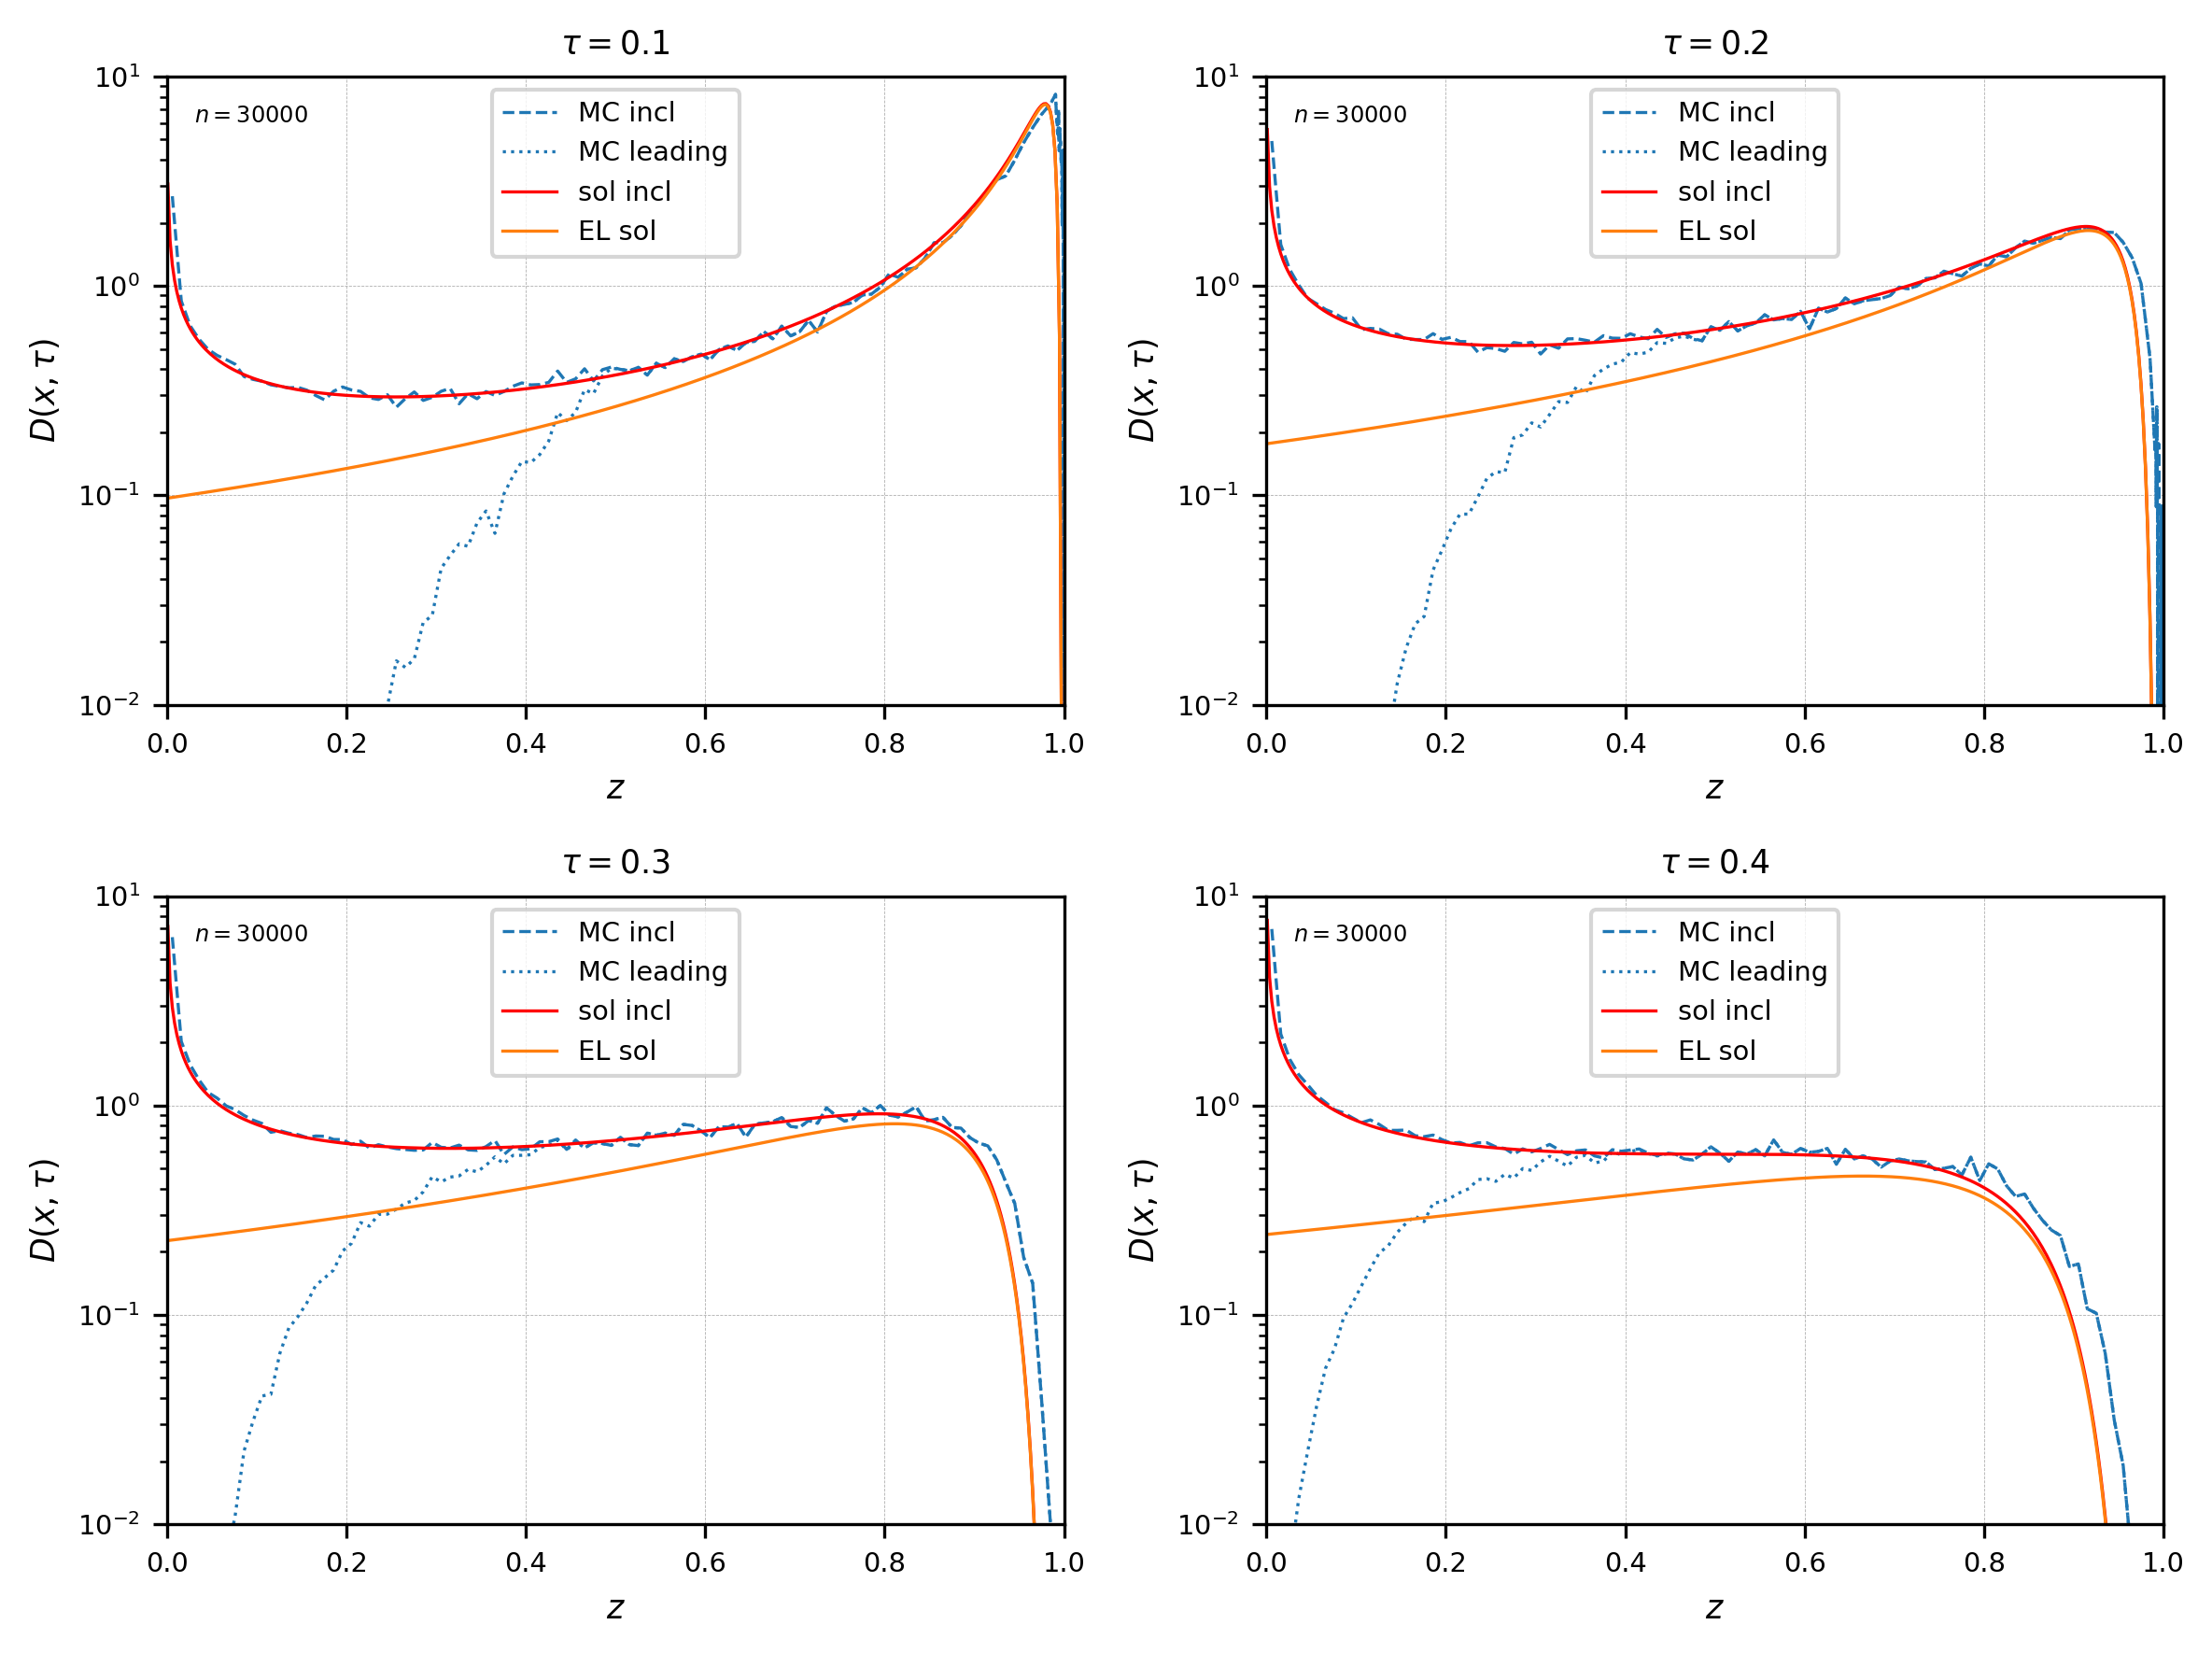
\includegraphics[width=13cm]{pictures/plots/distributions/leading/leading_medium_30k_lin.png}
    \caption{The inclusive energy distribution \(D(x,\tau)\) as generated by the Monte-Carlo program for gluons in medium. The dotted line indicates the leading parton of each shower. Plotted alongside the analytical solution of the kinetic rate equation \autoref{eqn: BDMPS_solution}, and the leading parton solution \autoref{eqn: leading_solution_supersimple1}. Simulated with \(n = 3\cdot 10^4\) showers, using \(\epsilon=10^{-3}\) and \(z_{\text{min}}=10^{-3}\).}
    \label{fig: leading_supersimple1}
\end{figure}

From \autoref{fig: leading_supersimple1} we can see that the solution given by \autoref{eqn: leading_solution_supersimple1} is a very good agreement for values of \(x>0,8\), and decent for values \(x>0,5\). This is expected as the energy-loss distribution \autoref{eqn: prob_energy_loss} assumes all emissions to be soft. It should however motivate us to find model for the energy-loss distribution able to deal with harder gluon emissions.

\subsection{Leading branches}\label{sec: leading_branches}
Before attempting to modify the current evolution equations, or crating a whole new set of equations for describing the leading parton evolution, we must know more about how the distribution behaves. A key question is whether the leading branch in a given splitting, generally yields the hardest parton at the end of the cascade. The simplest model imaginable is illustrated in \autoref{fig: leading_parton_same_branch} where the leading parton remains on the same branch for the entire evolution. In this scenario we could disregard the softest branch in every splitting, and just focus on the hardest branch.
\begin{figure}[H]
    \centering
    \begin{tikzpicture}
    \draw[dashed, opacity = 0.2] (2.5,-3.2) -- (2.5,3.2);
    \node[opacity =0.8] at (2.5,-3.5cm) {\(\tau_1\)};
    \draw[dashed, opacity = 0.2] (3.9,-3.2) -- (3.9,3.2);
    \node[opacity =0.8] at (3.9,-3.5cm) {\(\tau_2\)};
    \draw[dashed, opacity = 0.2] (5.3,-3.2) -- (5.3,3.2);
    \node[opacity =0.8] at (5.3,-3.5cm) {\(\tau_3\)};
    \draw[blue, dashed, opacity=0.9, line width = 0.15mm] (2.0cm,0) circle [x radius=0.1cm,y radius=0.4cm];
    \node[color = blue, opacity =0.8] at (2.0cm,0.6cm) {\(\mathcal{J}_0\)};
    \draw[blue, dashed, opacity=0.9, line width = 0.15mm] (3.5cm,0.9) circle [x radius=0.1cm,y radius=0.4cm];
    \node[color = blue, opacity =0.8] at (3.5cm,1.5cm) {\(\mathcal{J}_1\)};
    \draw[blue, dashed, opacity=0.9, line width = 0.15mm] (4.9cm,1.9) circle [x radius=0.1cm,y radius=0.4cm];
    \node[color = blue, opacity =0.8] at (4.9cm,2.5cm) {\(\mathcal{J}_2\)};
    \draw[blue, dashed, opacity=0.9, line width = 0.15mm] (6.3cm,2.75) circle [x radius=0.1cm,y radius=0.4cm];
    \node[color = blue, opacity =0.8] at (6.3cm,3.35cm) {\(\mathcal{J}_3\)};
    \begin{feynman}
            \vertex (a)  {};
            \vertex [right=2.5cm of a ] (a1);
            \vertex [above right=1.2cm and 1.4cm of a1] (b1);
            \vertex [below right=1.2cm and 1.4cm of a1] (b2);
            \vertex [above right=1.0cm and 1.4cm of b1] (c1);
            \vertex [below right=0.6cm and 1.4cm of b1] (c2);
            \vertex [above right=0.15cm and 1.4cm of b2] (c3);
            \vertex [below right=1.0cm and 1.4cm of b2] (c4);
            \vertex [above right=0.7cm and 1.4cm of c1] (d1){\(z_1\)};
            \vertex [below right=0.15cm and 1.4cm of c1] (d2){\(z_2\)};
            \vertex [above right=0.3cm and 1.4cm of c2] (d3){\(z_3\)};
            \vertex [below right=0.4cm and 1.4cm of c2] (d4){\(z_4\)};
            \vertex [right=0.7cm of c3] (d5);
            \vertex [above right=0.15cm and 1.4cm of c3] (d6){\(z_5\)};
            \vertex [above right=0.15cm and 1.4cm of c4] (d7){\(z_6\)};
            \vertex [below right=0.7cm and 1.4cm of c4] (d8){\(z_7\)};
            \diagram* {
            (a) -- [gluon, edge label  = {\small \(1.0\)}] (a1),
            (a1) -- [gluon, edge label = {\small \(0.9\)}] (b1),
            (b2) -- [gluon, edge label = {\small \(0.1\)}] (a1),
            (b1) -- [gluon, edge label = {\small \(0.88\)}] (c1),
            (c2) -- [gluon, edge label = {\small \(0.02\)}] (b1),
            (b2) -- [ghost, edge label = {\small \(0.02\)}] (c3),
            (b2) -- [gluon] (d6),
            (c4) -- [gluon, edge label = {\small \(0.08\)}] (b2),
            (c1) -- [gluon, edge label = {\small \(0.87\)}] (d1),
            (d2) -- [gluon, edge label = {\small \(0.01\)}] (c1),
            (c2) -- [gluon, edge label = {\small \(0.01\)}] (d3),
            (d4) -- [gluon, edge label = {\small \(0.01\)}] (c2),
            (c4) -- [gluon, edge label = {\small \(0.06\)}] (d7),
            (d8) -- [gluon, edge label = {\small \(0.02\)}] (c4),
            };
        \end{feynman}
\end{tikzpicture}
\caption{Illustration of the leading parton \(\mathcal{J}_{\tau_i}\) remaining on the same branch for the entire evolution. The leading parton is therefore on-branch.}
\label{fig: leading_parton_same_branch}
\end{figure}

The other scenario is illustrated in \autoref{fig: leading_parton_diff_branch}, where the leading parton at one time, is on a different branch than the leading parton at a later time. If this is how the evolution goes, it is important to keep track of every single branch following a splitting, to find the hardest parton. When the leading parton remains on the same branch throughout the cascade, we will call it \emph{on-branch}, when it changes branches we will call it \emph{off-branch}.
\begin{figure}[H]
    \centering
    \begin{tikzpicture}
    \draw[dashed, opacity = 0.2] (2.5,-3.2) -- (2.5,3.2);
    \node[opacity =0.8] at (2.5,-3.5cm) {\(\tau_1\)};
    \draw[dashed, opacity = 0.2] (3.9,-3.2) -- (3.9,3.2);
    \node[opacity =0.8] at (3.9,-3.5cm) {\(\tau_2\)};
    \draw[dashed, opacity = 0.2] (5.3,-3.2) -- (5.3,3.2);
    \node[opacity =0.8] at (5.3,-3.5cm) {\(\tau_3\)};
    \draw[blue, dashed, opacity=0.9, line width = 0.15mm] (2.0cm,0) circle [x radius=0.1cm,y radius=0.4cm];
    \node[color = blue, opacity =0.8] at (2.0cm,0.6cm) {\(\mathcal{J}_0\)};
    \draw[blue, dashed, opacity=0.9, line width = 0.15mm] (3.5cm,0.9) circle [x radius=0.1cm,y radius=0.4cm];
    \node[color = blue, opacity =0.8] at (3.5cm,1.5cm) {\(\mathcal{J}_1\)};
    \draw[blue, dashed, opacity=0.9, line width = 0.15mm] (4.9cm,-1.95) circle [x radius=0.1cm,y radius=0.4cm];
    \node[color = blue, opacity =0.8] at (4.9cm,-2.6cm) {\(\mathcal{J}_2\)};
    \draw[blue, dashed, opacity=0.9, line width = 0.15mm] (6.3cm,0.2) circle [x radius=0.1cm,y radius=0.4cm];
    \node[color = blue, opacity =0.8] at (6.3cm,-0.4cm) {\(\mathcal{J}_3\)};
    \begin{feynman}
            \vertex (a)  {};
            \vertex [right=2.5cm of a ] (a1);
            \vertex [above right=1.2cm and 1.4cm of a1] (b1);
            \vertex [below right=1.2cm and 1.4cm of a1] (b2);
            \vertex [above right=1.0cm and 1.4cm of b1] (c1);
            \vertex [below right=0.6cm and 1.4cm of b1] (c2);
            \vertex [above right=0.1cm and 1.4cm of b2] (c3);
            \vertex [below right=1.0cm and 1.4cm of b2] (c4);
            \vertex [above right=0.7cm and 1.4cm of c1] (d1){\(z_1\)};
            \vertex [below right=0.15cm and 1.4cm of c1] (d2){\(z_2\)};
            \vertex [above right=0.3cm and 1.4cm of c2] (d3){\(z_3\)};
            \vertex [below right=0.4cm and 1.4cm of c2] (d4){\(z_4\)};
            \vertex [right=0.7cm of c3] (d5);
            \vertex [above right=0.1cm and 1.4cm of c3] (d6){\(z_5\)};
            \vertex [above right=0.15cm and 1.4cm of c4] (d7){\(z_6\)};
            \vertex [below right=0.7cm and 1.4cm of c4] (d8){\(z_7\)};
            \diagram* {
            (a) -- [gluon, edge label  = {\small \(1.0\)}] (a1),
            (a1) -- [gluon, edge label = {\small \(0.6\)}] (b1),
            (b2) -- [gluon, edge label = {\small \(0.4\)}] (a1),
            (b1) -- [gluon, edge label = {\small \(0.35\)}] (c1),
            (c2) -- [gluon, edge label = {\small \(0.25\)}] (b1),
            (b2) -- [ghost, edge label = {\small \(0.02\)}] (c3),
            (b2) -- [gluon] (d6),
            (c4) -- [gluon, edge label = {\small \(0.38\)}] (b2),
            (c1) -- [gluon, edge label = {\small \(0.23\)}] (d1),
            (d2) -- [gluon, edge label = {\small \(0.22\)}] (c1),
            (c2) -- [gluon, edge label = {\small \(0.01\)}] (d3),
            (d4) -- [gluon, edge label = {\small \(0.24\)}] (c2),
            (c4) -- [gluon, edge label = {\small \(0.16\)}] (d7),
            (d8) -- [gluon, edge label = {\small \(0.22\)}] (c4),
            };
        \end{feynman}
\end{tikzpicture}
\caption{Illustration of the leading parton \(\mathcal{J}_{\tau_i}\) changing what branch it on during the evolution, due to splittings where \(z\rightarrow 0.5\). The leading is parton at the end of the evolution is therefore off-branch.}
\label{fig: leading_parton_diff_branch}
\end{figure}

There is no precise formulation for how often the leading parton is off-branch, so it could be interesting to determine this by using our Monte-Carlo program for gluons in medium. This is implemented by picking the hardest parton at the end of the shower, and then iterating backwards through the evolution, to check that the hardest parton is the hardest leg of each splitting. The resulting plot for several different values of \(\tau\), where the leading on-branch partons are plotted separately from the leading off-branch partons, is given in \autoref{fig: leading_scaling}. 
\begin{figure}[htb]
    \centering
    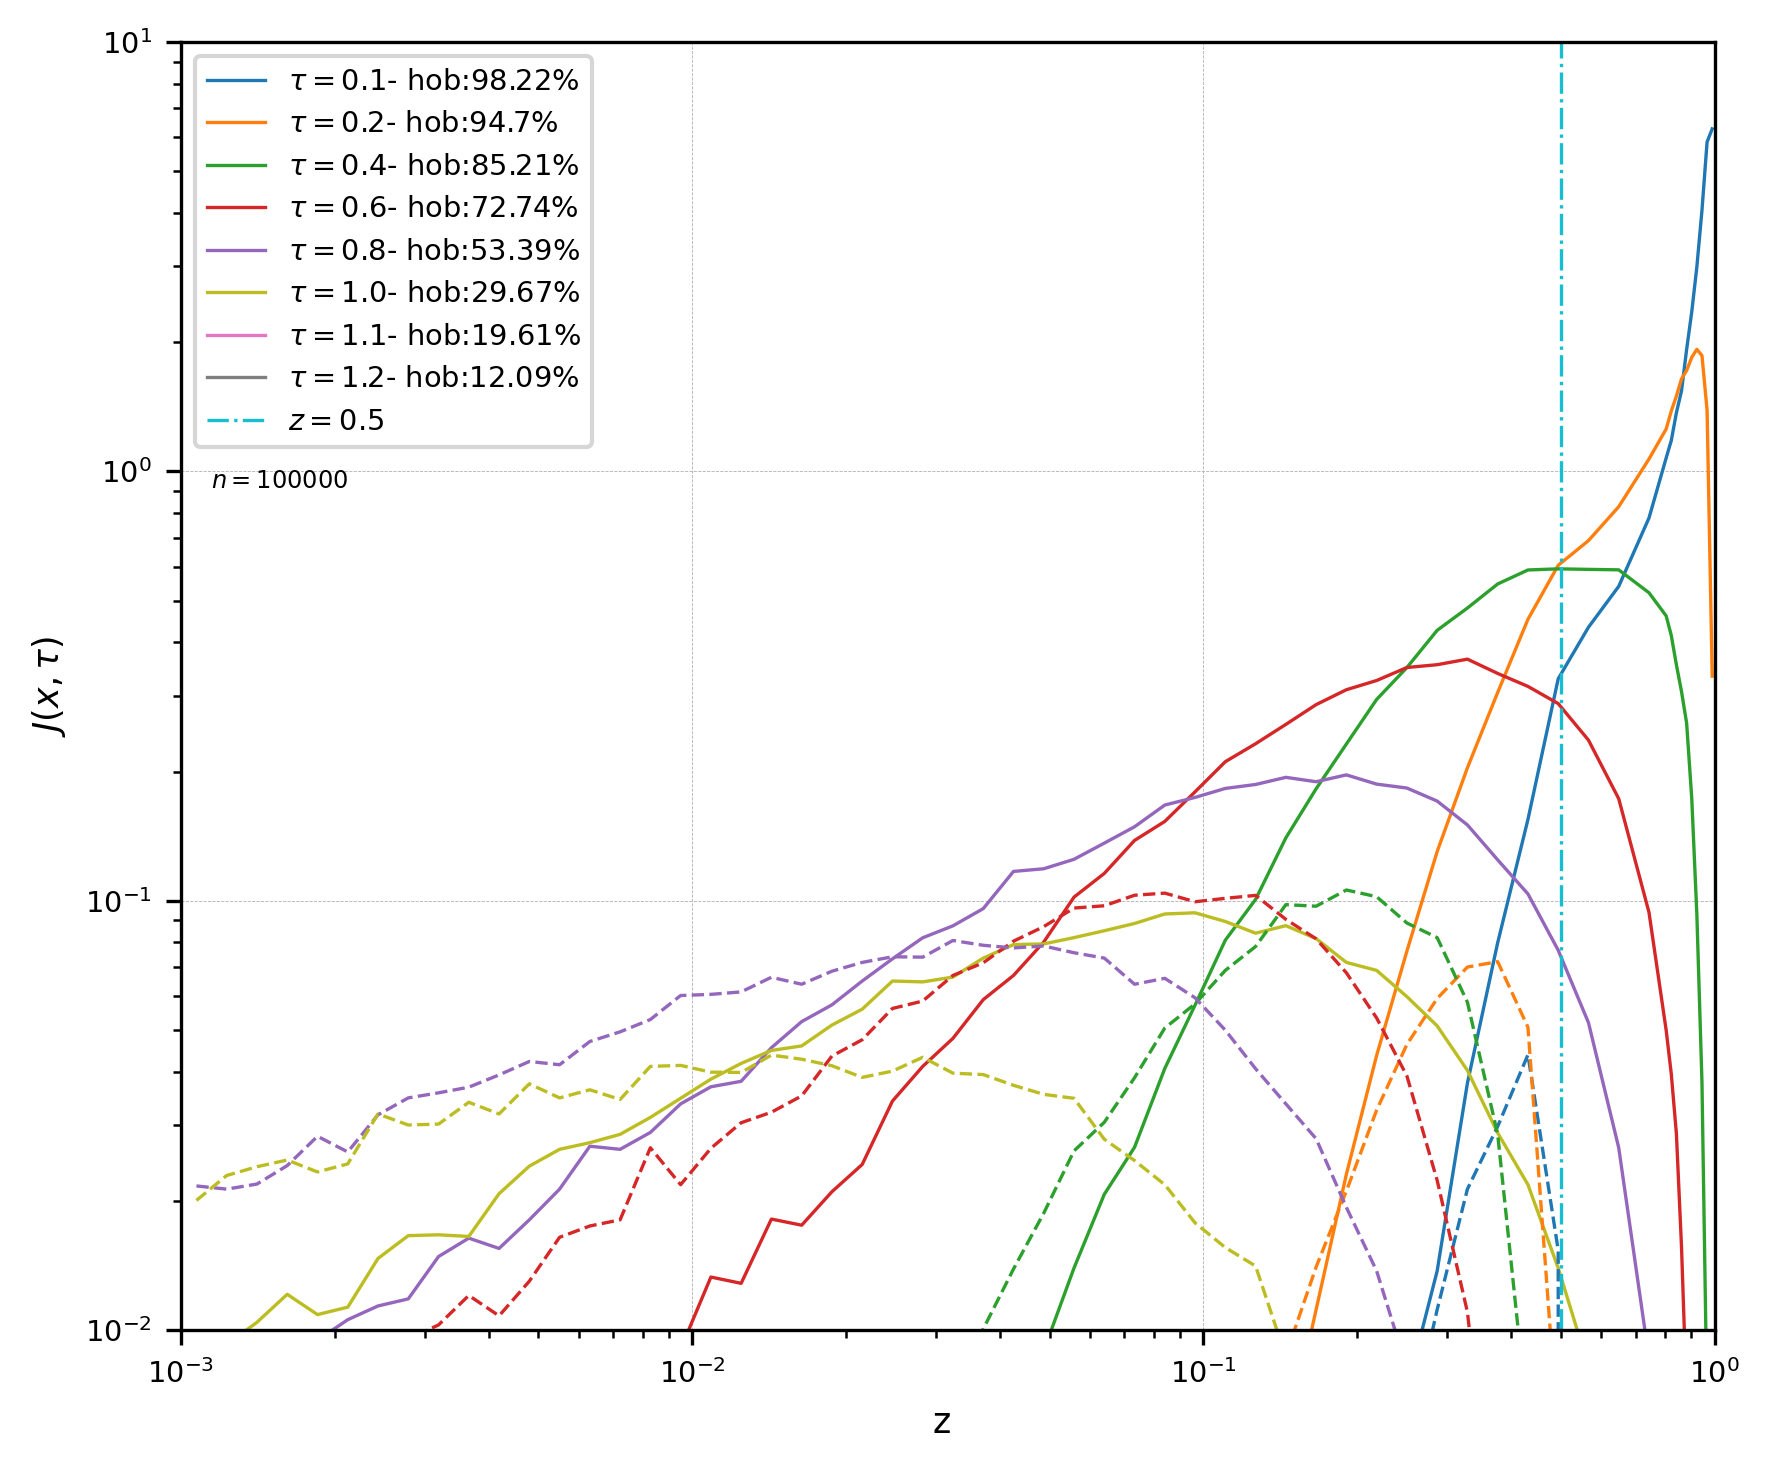
\includegraphics[width=12cm]{pictures/plots/distributions/leading/leading_scaling_100k.png}
    \caption{Leading partons of the medium cascade. The solid lines indicate that the leading parton is on-branch, while the dashed lines indicate that the leading parton is off-branch. Percentages of total number of leading partons on-branch for each value of \(\tau\) is given in the legend. Simulated with \(n=10^{5}\) showers, using \(\epsilon=10^{-3}\) and \(z_{\text{min}}=10^{-3}\).Some of the values for \(\tau\) are excluded from the plot, to make it more readable, but the percentages of hob (hardest on branch) is still given in the legend.}
    \label{fig: leading_scaling}
\end{figure}

There are several notable results in \autoref{fig: leading_scaling}. Firstly, the off-branch leading partons are all confined to \(z\lessapprox 0,5\). This is expected, since the shower requires either a splitting \(z\sim 0,5\) for the leading parton to change branches during the evolution, or a very long evolution such that all partons are moving towards small values of \(x\). The second property to note is how the percentage of leading on-branch partons, changes with the values of \(\tau\). This can be made more explicit my creating a plot of the fraction of on-branch leading partons, for a shower with given \(\tau\), as presented in \autoref{fig: leading_polyfit} with a second degree polynomial fit.
\begin{figure}[htb]
    \centering
    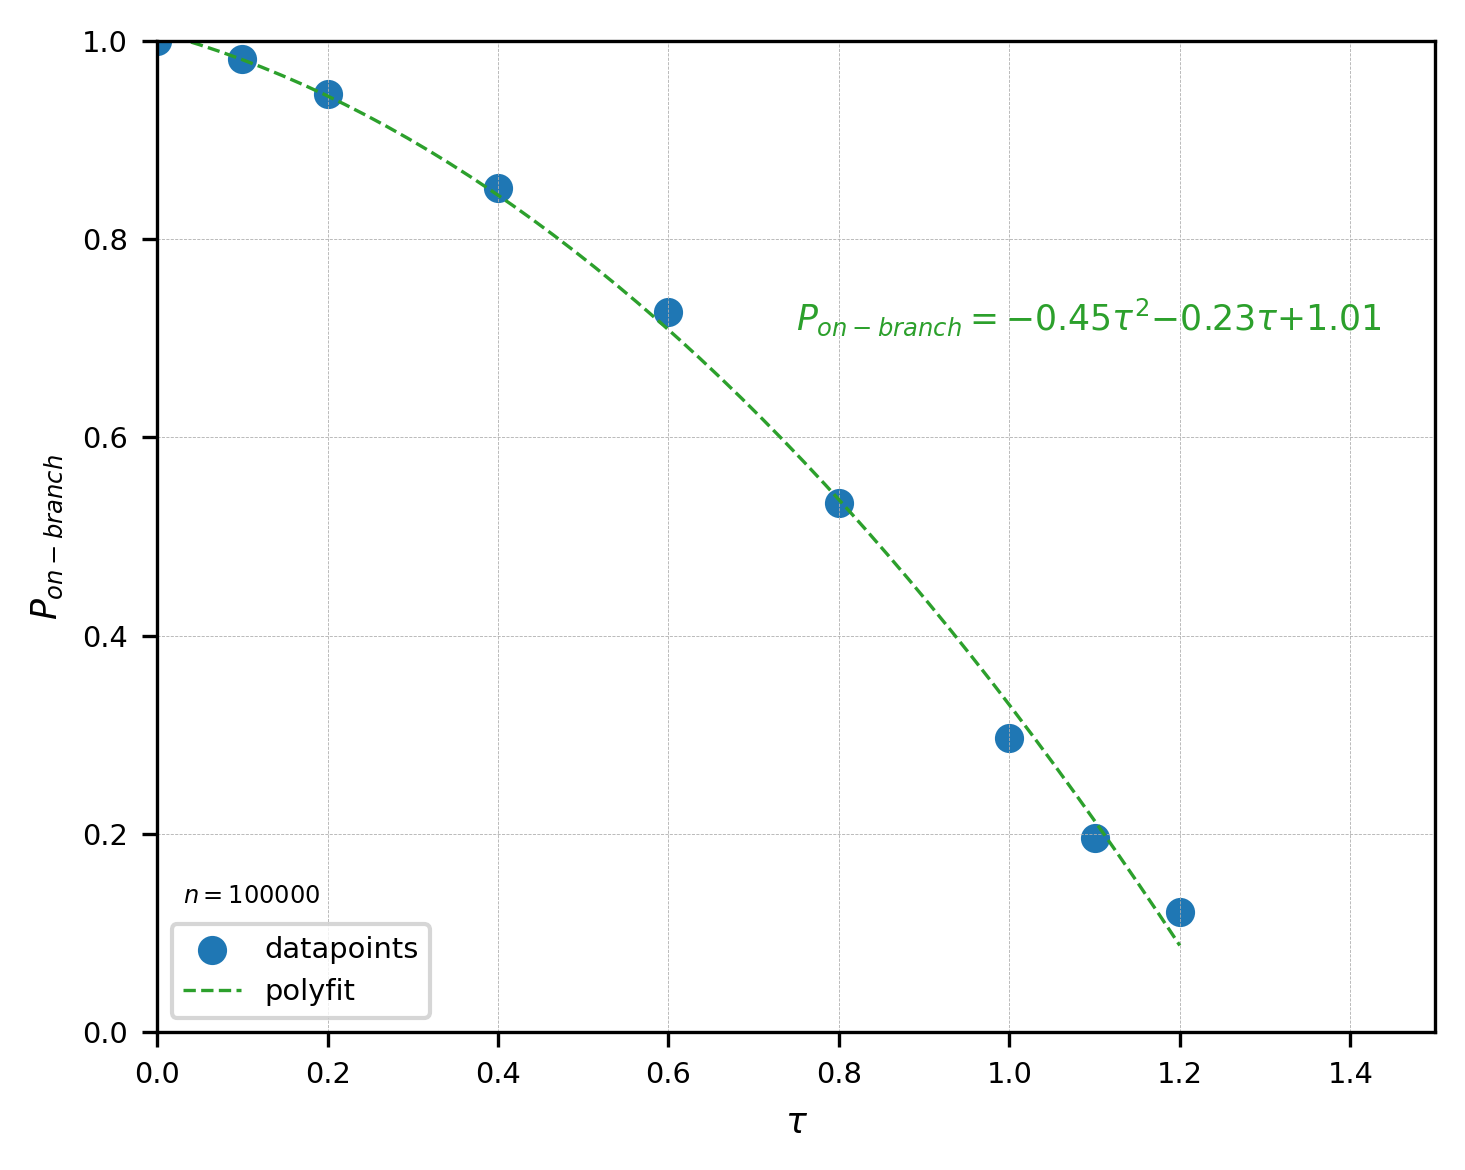
\includegraphics[width=10cm]{pictures/plots/distributions/leading/leading_onbranch_polyfit_100k.png}
    \caption{Polyfit of the fraction of leading partons which are on-branch, for a shower with a given \(\tau\) value. The dataset used is the same as for \autoref{fig: leading_scaling}; simulated with \(n=10^{5}\) showers, using \(\epsilon=10^{-3}\) and \(z_{\text{min}}=10^{-3}\).}
    \label{fig: leading_polyfit}
\end{figure}

It is therefore important to take into account how often off-branch leading partons is expected when creating a new model for the evolution of the leading parton distribution. For small values of \(\tau\), where off-branch leading partons is rare, it can be viable to exclusively follow the leading parton in each vertex. For larger evolutions it is however necessary to take into account these off-branch leading partons.

\subsection{Leading parton evolution equations in vacuum}
When looking at \autoref{fig: vacuum_distribution_quark_and_gluon} which was generated for quarks and gluons in the vacuum cascade, there is an interesting observation to be made. The distribution of the leading parton is identical to the inclusive distribution for values of \(z>0.5\). This implies that the information we are looking for is already contained within the evolution equations - which makes sense as they are resumming all splittings which may occur. This should motivate us to make some adjustments to the current evolution equations, such that they follow exclusively the leading parton.

\subsubsection*{Derivation}
In \autoref{sec: leading_branches} we saw that the leading parton is predominantly on-branch up to values of \(\tau \sim 0.5\). Keeping this in mind, we can attempt to find an alternate formulation of the evolution equations in vacuum, where we follow exclusively the leading parton in each vertex, and be confident of where these results should be valid.

The equations can be constructed in a manner similar to the DGLAP equation which we constructed in \autoref{app: DGLAP_derivation}, using generating functionals. We start with the functional \(\mathcal{Z}(p,t=0) = u(p)\), with the property \(\frac{\delta u(p)}{\delta u(k)} = u(1-\frac{k}{p})\), and normalization \(\mathcal{Z}(p)|_{u=1} = 1\)
\begin{align}\label{eqn: Leading_GF1}
    \frac{\partial}{\partial t} \mathcal{Z}(p,t) = \int_0^1 dz \, P(z) \mathcal{Z}(zp)\mathcal{Z}((1-z)p) - \int_0^1 dz\, P(z) \mathcal{Z}(p)
\end{align}
but now we wish to adjust this to account for the leading partons, by changing the integration limits \(0\rightarrow 1/2\) and \(1/2\rightarrow 1\). The real term of \autoref{eqn: Leading_GF1} can then be written as
\begin{align}
    \mathbb{R} &= \int_0^{1/2} dz \, P(z) \mathcal{Z}(zp)\mathcal{Z}((1-z)p) + \int_{1/2}^1 dz \, P(z) \mathcal{Z}(zp)\mathcal{Z}((1-z)p)
\end{align}
and we are only interested in retaining the leading particle with \(z>1/2\),
\begin{align}
    \mathbb{R} &= \int_0^{1/2} dz \, P(z) u(zp)\mathcal{Z}((1-z)p) + \int_{1/2}^1 dz \, P(z) \mathcal{Z}(zp)u((1-z)p).
\end{align}
Since we are still working with gluons we can use \(P_{gg}(z) = P_{gg}(1-z)\), and use a change of variable \(z'=1-\), to write
\begin{align}
    \mathbb{R} &= \int_0^{1/2} dz \, P(z) u(zp)\mathcal{Z}((1-z)p) - \int_{1/2}^0 dz \, P(z') \mathcal{Z}((1-z')p)u(z'p) \nonumber\\
    &= 2\int_0^{1/2} dz \, P(z) u(zp)\mathcal{Z}((1-z)p) 
\end{align}
then taking the functional derivative,
\begin{align}
    \frac{\delta \mathbb{R}}{\delta u(k)}|_{u=1} &= 2\int_0^{1/2} dz \, P(z) \left[\frac{\delta u(zp)}{\delta u(k)}|_{u=1} \mathcal{Z}((1-z)p)|_{u=1} + u(zp)|_{u=1} \frac{\delta \mathcal{Z}((1-z)p)}{\delta u(k)}|_{u=1} \right] \nonumber \\
    &= 2\int_0^{1/2} dz \, P(z) \left[\delta(1-\frac{x}{z}) + D(\frac{x}{1-z},t) \right].
\end{align}
Being careful with the limits in the second term as we are requiring that \(x<1-z \rightarrow z<1-x\) in the distribution, as well as \(z<1/2\) from the integral. Bringing both of these explicitly into the integral, and again introducing \(\tilde{P}(z) = 2 P(z)\) we can write
\begin{equation}
    \frac{\delta \mathbb{R}}{\delta u(k)}|_{u=1} = \int_0^{1/2} dz \, \tilde{P}(z) \delta(1-\frac{x}{z}) + \int_0^{\text{min}(\frac{1}{2}, 1-x)} dz \, \tilde{P}(z) D(\frac{x}{1-z},t).
\end{equation}
In the first term there is a criteria from the delta function that \(x=z\), that means the real term can be rewritten using a step function \( \Theta(x<\frac{1}{2})\),
\begin{equation}\label{eqn: leading_GF_real}
    \frac{\delta \mathbb{R}}{\delta u(k)}|_{u=1} = \Theta(x<\frac{1}{2})x \tilde{P}(x) + \int_0^{\text{min}(\frac{1}{2}, 1-x)} dz \, \tilde{P}(z) D(\frac{x}{1-z},t)
\end{equation}
and a similar treatment can be given for the virtual term, 
\begin{align}\label{eqn: leading_GF_virtual}
    \frac{\delta \mathbb{V}}{\delta u(k)}|_{u=1} &= -\int_0^{1/2}dz\, \tilde{P}(z) \frac{\delta \mathcal{Z}(p)}{\delta u(k)}|_{u=1} \nonumber \\
    &= -\int_0^{1/2}dz\, \tilde{P}(z) D(x,t).
\end{align}
Using \autoref{eqn: leading_GF_real} and \autoref{eqn: leading_GF_virtual}, we can write \autoref{eqn: Leading_GF1} as
\begin{align}\label{eqn: leading_vacuum_evolutionequation}
    \begin{split}
    \frac{\partial}{\partial t} D(x,t) &= \Theta(x<\frac{1}{2})x \tilde{P}(x) + \int_0^{\text{min}(\frac{1}{2}, 1-x)} dz \, \tilde{P}(z) D(\frac{x}{1-z},t) -\int_0^{1/2}dz\, \tilde{P}(z) D(x,t).
    \end{split}
\end{align}
\autoref{eqn: leading_vacuum_evolutionequation} is therefore now a proposed evolution equation for the leading parton of pure gluon cascades in medium, where the leading parton is assumed to be on-branch.

\subsubsection*{Writing the equation in Mellin space}
We will now attempt to solve \autoref{eqn: leading_vacuum_evolutionequation}. Starting by making a change of variables \(z'=1-z\) in the gain term
\begin{align}
    \begin{split}
    \frac{\partial}{\partial t} D(x,t) &= \Theta(x<\frac{1}{2})x \tilde{P}(x) \\
    &\quad + \int_{\text{min}(\frac{1}{2}, x)}^{1} dz' \, \tilde{P}(z') D(\frac{x}{z'},t) - \int_{1/2}^1 dz'\, \tilde{P}(z') D(x,t).
    \end{split}
\end{align}
and the \(z'\)s can for simplicity be written as \(z\). Performing the Mellin transform defined in \autoref{eqn: mellin_transforms}
\begin{align}
    \begin{split}
    \frac{\partial}{\partial t} \tilde{D}(\nu,t) &= \int_0^1 dx\, x^{\nu-1} \Theta(x<\frac{1}{2})x \tilde{P}(x) \\
    &\quad + \int_0^1 dx\, x^{\nu-1} \int_{\text{min}(\frac{1}{2}, x)}^{1} dz \, \tilde{P}(z) D(\frac{x}{z},t) -\int_{1/2}^1dz\, \tilde{P}(z) \tilde{D}(\nu,t)
    \end{split}
\end{align}
and splitting up the integrals in the gain term for values of \(x<1/2\) and \(x>1/2\),
\begin{align}
    \begin{split}
    \frac{\partial}{\partial t} \tilde{D}(\nu,t) &= \int_0^{1/2} dx\, x^{\nu-1} x \tilde{P}(x) \\
    &\quad + \int_0^{1/2} dx\, x^{\nu-1} \int_{1/2}^{1} dz \, \tilde{P}(z) D(\frac{x}{z},t) -\int_{1/2}^1dz\, \tilde{P}(z) \tilde{D}(\nu,t) \\
    &\quad + \int_{1/2}^1 dx\, x^{\nu-1} \int_{x}^{1} dz \, \tilde{P}(z) D(\frac{x}{z},t).
    \end{split}
\end{align}
Changing the integration limits in the third line such that 
\(\int_{1/2}^1dx \int_x^1 dz \Rightarrow \int_{1/2}^1 dz \int_{1/2}^z dx  \) 
\begin{align}
    \begin{split}
    \frac{\partial}{\partial t} \tilde{D}(\nu,t) &= \int_0^{1/2} dx\, x^{\nu-1} x \tilde{P}(x) \\
    &\quad + \int_0^{1/2} dx\, x^{\nu-1} \int_{1/2}^{1} dz \, \tilde{P}(z) D(\frac{x}{z},t) -\int_{1/2}^1dz\, \tilde{P}(z) \tilde{D}(\nu,t) \\
    &\quad + \int_{1/2}^{1} dz \, \tilde{P}(z) \int_{1/2}^z dx\, x^{\nu-1} D(\frac{x}{z},t)
    \end{split}
\end{align}
and then performing a change of variable in the gain terms such that \(\xi = x/z \quad \Rightarrow \quad dx = z d\xi\)
\begin{align}
    \begin{split}
    \frac{\partial}{\partial t} \tilde{D}(\nu,t) &= \int_0^{1/2} dx\, x^{\nu-1} x \tilde{P}(x) \\
    &\quad + \int_{1/2}^{1} dz \, \tilde{P}(z) \int_0^{1/2z} (zd\xi)\, (z\xi)^{\nu-1} D(\xi,t) -\int_{1/2}^1dz\, \tilde{P}(z) \tilde{D}(\nu,t) \\
    &\quad + \int_{1/2}^{1} dz \, \tilde{P}(z) \int_{1/2z}^1 (zd\xi)\, (z\xi)^{\nu-1} D(\xi,t).
    \end{split}
\end{align}
It is then possible to merge the integration limits with respect to \(d\xi\) again and perform the Mellin transform on \(D(\xi,t)\)
\begin{align}
    \begin{split}
    \frac{\partial}{\partial t} \tilde{D}(\nu,t) &= \int_0^{1/2} dx\, x^{\nu-1} x \tilde{P}(x) \\
    &\quad + \int_{1/2}^{1} dz \, \tilde{P}(z) z^\nu \tilde{D}(\nu,t) -\int_{1/2}^1dz\, \tilde{P}(z) \tilde{D}(\nu,t) 
    \end{split}
\end{align}
which can be written as a non-homogeneous differential equation
\begin{align}
    \begin{split}
    \frac{\partial}{\partial t} \tilde{D}(\nu,t) &= 2\int_0^{1/2} dx\, \frac{x^{\nu-1}}{(1-x)} + 2\int_{1/2}^{1} dz \, \left( \frac{z^\nu-1}{z(1-z)}\right) \tilde{D}(\nu,t).
    \end{split}
\end{align}
For simplicity we can introducing the incomplete beta function \(\mathrm{B}_{\frac{1}{2}}(\nu,0)\)
\begin{align}\label{eqn: leading_parton_vacuum_diferentialequationsolution}
    \begin{split}
    \frac{\partial}{\partial t} \tilde{D}(\nu,t) &= 2 \, \mathrm{B}_{\frac{1}{2}}(\nu,0) + 2\int_{1/2}^{1} dz \, \left( \frac{z^\nu-1}{z(1-z)}\right) \tilde{D}(\nu,t).
    \end{split}
\end{align}

\subsubsection*{Solving the equation in Mellin space}
We will now solve \autoref{eqn: leading_parton_vacuum_diferentialequationsolution}, with the initial condition \(\tilde{D}(\nu, 0) =1\). Writing the equation in a general form
\begin{align}\label{eqn: leading_simplediff}
    s'(\nu,t) - p(\nu) s(\nu,t) &= f(\nu)
\end{align}
where
\begin{align}\label{eqn: leading_fullfunctions_definitions}
    \begin{split}
    s(\nu,t) &= \tilde{D}(\nu,t) \\
    s'(\nu,t) &= \frac{\partial}{\partial t}\, \tilde{D}(\nu,t) \\
    p(\nu) &= 2\int_{1/2}^{1} dz \, \left( \frac{z^\nu-1}{z(1-z)}\right) \\
    f(\nu) &= 2 \, \mathrm{B}_{\frac{1}{2}}(\nu,0),
    \end{split}
\end{align}
then the solution of the corresponding homogeneous system \(h'(\nu,t) - p(\nu) h(\nu,t) = 0\), with with the initial condition \(h(\nu,0) = 1\),
\begin{align}
    h(\nu,t) &= - \frac{f(\nu)}{p(\nu)} \, \exp\left(p(\nu) \,t\right). 
\end{align}
By variation of parameters we are looking for a solution \(s(\nu,t)\) of the non-homogeneous system
\begin{align}
    s(\nu, t) &= v(t) \, h(\nu, t),
\end{align}
which is obtained by finding a function \(v(t)\) such that \(v'(t)h(\nu,t) = f(\nu)\).
\begin{align}
    v(t) &= \int \frac{f(\nu)}{h(\nu, t)} dt
    %&= -\int p(\nu) \, \exp\left(-p(\nu) \,t\right)\; dt \nonumber \\
    = \exp\left(-p(\nu) \,t\right) + C
\end{align}
and the solution \(s(\nu,t)\) is therefore
\begin{align}
    s(\nu,t) &= v(t) \, h(\nu, t)
    %&= \left( \exp\left(-p(\nu) \,t\right) +C \right) \left(- \frac{f(\nu)}{p(\nu)} \, \exp\left(p(\nu) \,t\right) \right)   \nonumber \\
    = -C\,\frac{f(\nu)}{p(\nu)}\, \exp(p(\nu)t) - \frac{f(\nu)}{p(\nu)}.
\end{align}
determining \(C\) from the initial condition we get the final solution 
\begin{align}\label{eqn: leading_simplediff_solution}
    s(\nu,t) &= \frac{f(\nu)+p(\nu)}{p(\nu)}\, \exp(p(\nu)t) - \frac{f(\nu)}{p(\nu)},
\end{align}
which can be verified by inserting \autoref{eqn: leading_simplediff_solution} into \autoref{eqn: leading_simplediff}. Inserting the full functions defined in \autoref{eqn: leading_fullfunctions_definitions} we obtain, 
\begin{align}\label{eqn: leading_vacuum_solution_mellinspace}
    \begin{split}
    \tilde{D}(\nu,t) &= \frac{\mathrm{B}_{\frac{1}{2}}(\nu,0)+\int_{1/2}^{1} dz \, \left( \frac{z^\nu-1}{z(1-z)}\right)}{\int_{1/2}^{1} dz \, \left( \frac{z^\nu-1}{z(1-z)}\right)}\, \exp(2\int_{1/2}^{1} dz \, \left( \frac{z^\nu-1}{z(1-z)}\right)\, t) \\
    &\quad - \frac{\mathrm{B}_{\frac{1}{2}}(\nu,0)}{\int_{1/2}^{1} dz \, \left( \frac{z^\nu-1}{z(1-z)}\right)}
    \end{split}
\end{align}

\subsubsection*{Discussing the solution in Mellin space}
Performing the inverse Mellin transform on the solution obtained in \autoref{eqn: leading_vacuum_solution_mellinspace} is not straightforward. To gain a clearer picture of why, we can plot the solution of the leading parton distribution, against the solution of the DGLAP equation \autoref{eqn: DGLAP_solution_mellinspace}, in Mellin space. Note that this is not the final solution of the DGLAP equation, but the one obtained in Mellin space, before transforming back to momentum space. The resulting plot is given in \autoref{fig: mellin_solutions} 
\begin{figure}[htb]
    \centering
    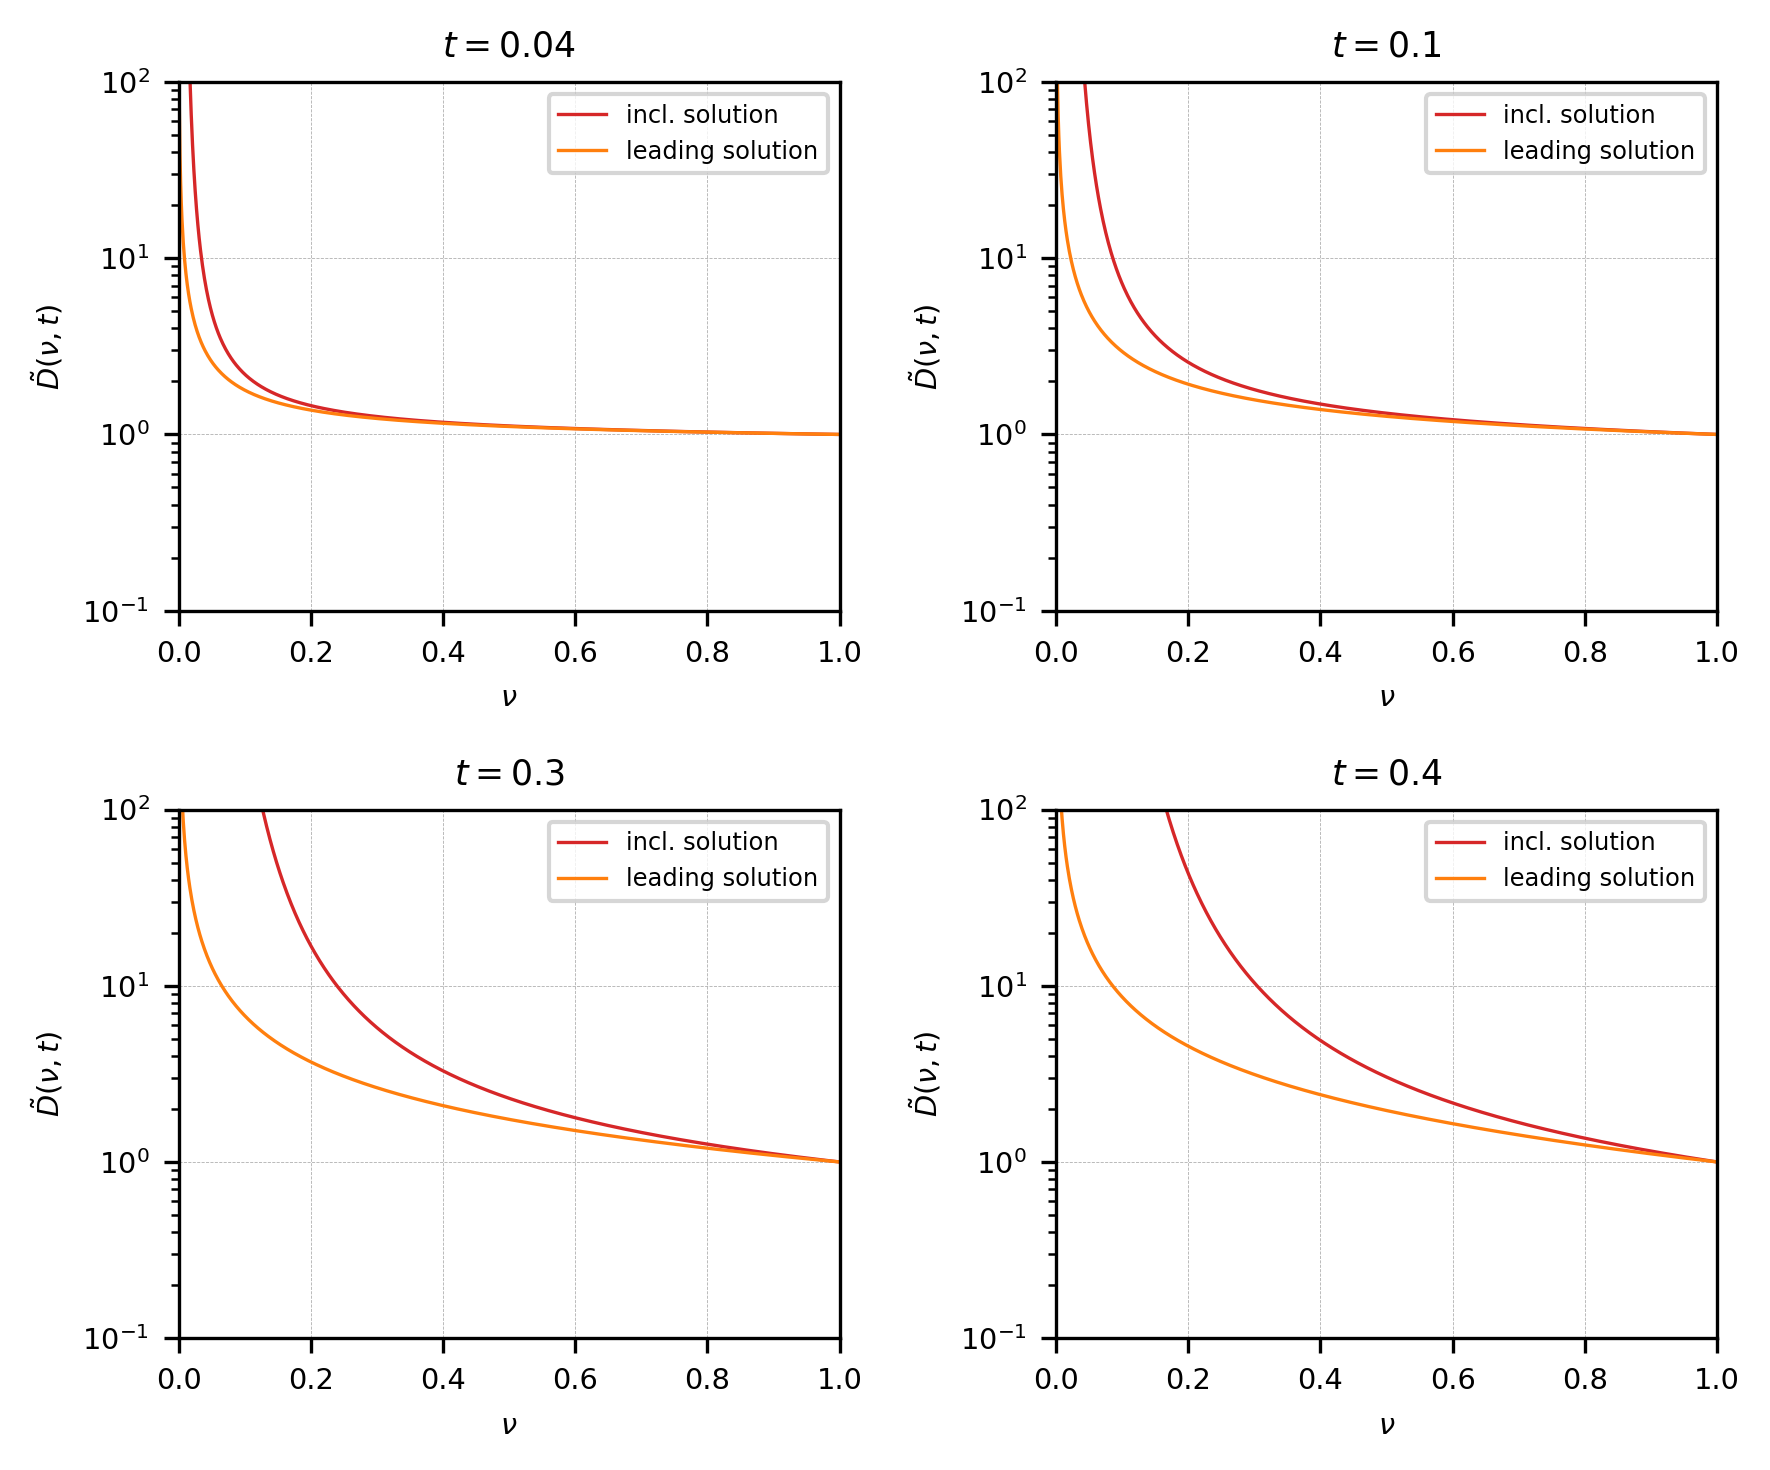
\includegraphics[width=12cm]{pictures/plots/misc/mellin_solutions.png}
    \caption{The solution of the leading parton evolution equations, for gluons in vacuum, in Mellin space as given by \autoref{eqn: leading_vacuum_solution_mellinspace} (orange), and the solution of the DGLAP equation as obtained in Mellin space as given by \autoref{eqn: DGLAP_solution_mellinspace} (red). The behavior at small \(\nu\) values is compared in the plot. For \(\nu>1\) they behave in the same manner.}
    \label{fig: mellin_solutions}
\end{figure}

When examining the plot it is worth noting that the general form is remarkably similar for values \(\nu<1\), and if the limits of the plot were expanded we would see that the behavior at \(\nu>1\) is identical. This is roughly what we would expect, as our proposed leading parton evolution equations are very similar in form to the DGLAP equation, with some modifications to the \(z\) limits. 

It should then be made explicit that the solution presented in \autoref{eqn: leading_vacuum_solution_mellinspace} is a function of \(\nu\) in Mellin space, and it needs to be transformed to momentum space to have proper interpretation. This may be possible by employing the Mellin transforms relation to other transformations such as the Laplace or Fourier transforms. Otherwise, an altogether different set of transformations and change of variables may be able to find a solution in momentum space.


\end{document}